
Desde 1980 hasta fines de 1990 los diseñadores se enfocaron en el diseño de software de la misma manera que lo habían hecho con el resto de los materiales. \vskip
Cuando se diseña para producir un objeto tangible, se necesita tener muy claro lo que se hace antes de iniciar la producción física, porque la producción es costosa, es costoso poner en marcha una fábrica para producir bienes físicos. \vskip En el ámbito del desarrollo de software, los diseñadores tuvieron que enfrentar nuevos retos, descubrir los nuevos medios y, a medida que lo hacían, aparecían nuevas especialidades, como el diseño de interacción o la arquitectura de información. Sin embargo, en esa época la práctica de los diseñadores apenas cambió. Todavía diseñaban los productos de manera tradicional, con mucho detalle y por adelantado, porque había un proceso de ``fabricación": había que hacer copias de los trabajo en discos flexibles y CDs y distribuirlas de la misma manera en la que se distribuyen los bienes físicos. Cometer errores en ese contexto se traducía en enormes costos de producción. \vskip

Internet cambió la lógica de distribución de software de una manera radical, la mayoría del software hoy en día se distribuye en línea y al desaparecer el proceso físico de fabricación se puede trabajar con ciclos de producción mucho más cortos.\vskip
Sin embargo el porcentaje de fracazos en los proyectos de software es notable, a continuación se realiza un análisis sobre este hecho:

\subsection{Análisis sobre fracazos y éxitos de los proyectos TI}
El informe del Caos en inglés \textit{Chaos Report} es publicado desde 1994 y cada dos años por la agencia de investigación ``Standish Group"\footnote{\url{https://www.standishgroup.com/}}, dando una visión sobre el fracaso o éxito de los proyectos en el sector de las TI, en inglés \textit{Information Technology} (IT). Para el informe del año 2015 se analizaron aproximadamente 50.000 proyectos de todo el mundo, desde mantenimientos pequeños hasta gigantescos proyectos de reingeniería.\vskip
Los proyectos se clasifican de la siguiente manera:
\begin{itemize}
    \item \textbf{Exitosos}: Son aquellos en los que no hay duda de que fueron un éxito.
    \item \textbf{Discutidos}: Son aquellos en los que hay dudas sobre si tuvieron éxito o fueron un fracaso
    \item \textbf{Fallidos}: Son aquellos en los que no hay duda de que fueron un fracaso
\end{itemize}

El éxito de estos proyectos se mide de acuerdo a tres variables:

\begin{itemize}
    \item \textbf{Acabado en plazos}.
    \item \textbf{Acabado en presupuesto}.
    \item Y \textbf{con resultados satisfactorios} (en el 2015 se elimina el ``Acabado en alcance” dada la necesaria variabilidad del mismo en el sector, recalculándose los cinco años anteriores con este criterio).
\end{itemize}

A continuación se pueden ver las cifras calculadas en el informe desde el 2011 al 2015.

%\begin{center}
% \begin{tabular}{ c | p{2cm} p{2cm} p{2cm} p{2cm} p{2cm} } 
%   \empty & 2011 & 2012 & 2013 & 2014 & 2015  \\ 
%   \hline
 %  Exitosos & 29\% & 27\% & 31\% & 28\% & 29\%  \\
 %  \hline
 %  Discutidos & 49\% & 56\% & 50\% & 55\% & 52\%   \\
%   \hline
 %  Fallidos & 22\% & 17\% & 19\% & 17\% & 19\% \\
%   \hline
  
%\end{tabular}
%\end{center}

\begin{figure}[h]
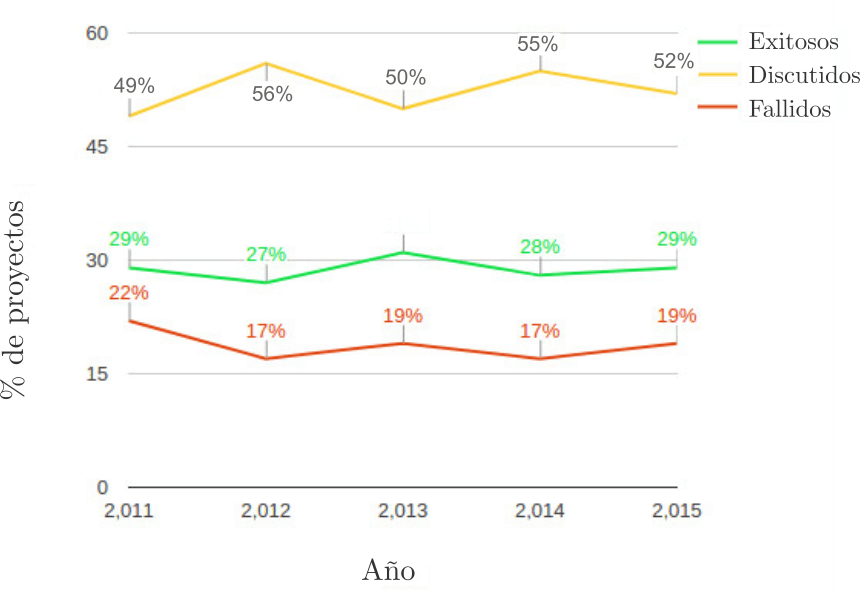
\includegraphics[width=11cm]{Img/Desarrollo/caos0.png}
\centering
\caption{\textbf{ \footnotesize{Proyectos, exitosos, discutidos y fallidos de 2011 hasta el 2015}}}
\label{fig:caos0}
\end{figure}

Lo primero que sorprende de esta comparativa es que del total de proyectos no hay ninguna tendencia en el éxito, se muestra oscilante sobre los mismos valores: el éxito entorno al 29\%, los discutidos entorno al 50\% y los fallidos entorno al 19\%. 

Hay otros factores para analizar que afectan al éxito o fracaso de los proyectos. Si se segmenta el informe por el tamaño de los proyectos como se puede apreciar en la Figura \ref{fig:caos1} , el resultado es claro e incluso esperado.
Se muestran los proyectos exitosos desde 2011 a 2015 desde la perspectiva del tamaño. El dato es muy significativo y confirma que más del 62\% de los proyectos exitosos son pequeños. Está claro que los proyectos grandes son exponencialmente más complejos que los proyectos pequeños y los proyectos gigantes son prácticamente imposibles de controlar.

\begin{figure}[h]
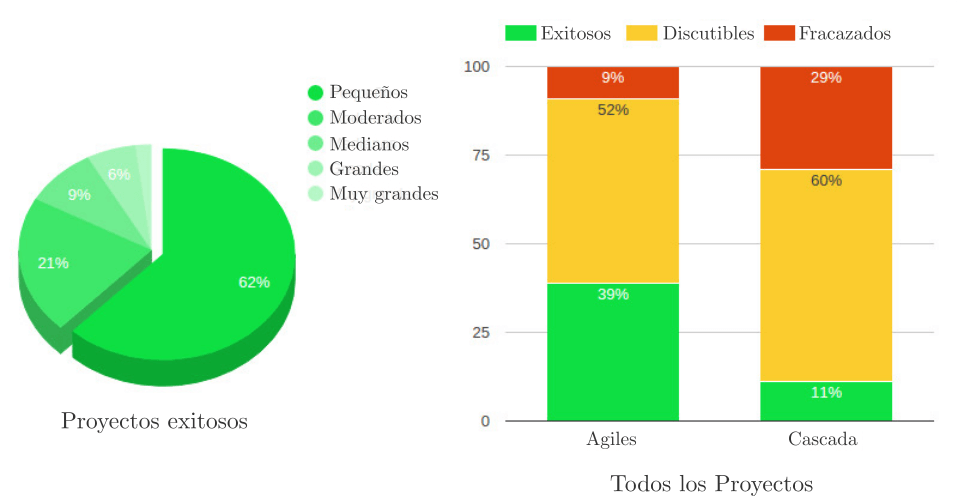
\includegraphics[width=15cm]{Img/Desarrollo/caos1.png}
\centering
\caption{\textbf{ \footnotesize{Éxito de los proyectos según su tamaño y métricas según la metodología.}}}
\label{fig:caos1}
\end{figure}

Otra información interesante que ofrece el Chaos Report es la comparativa del éxito de los proyectos en función de la metodología seguida para su desarrollo: \textit{ágil vs cascada}.

\begin{figure}[h]
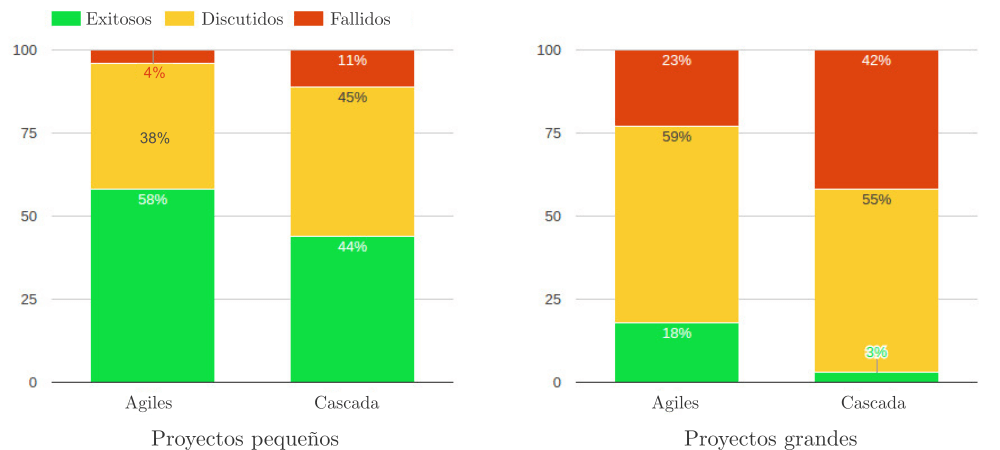
\includegraphics[width=15cm]{Img/Desarrollo/caos2.png}
\centering
\caption{\textbf{ \footnotesize{Métricas de los proyectos según la metodología.}}}
\label{fig:caos2}
\end{figure}

En los proyectos pequeños la diferencia no es tan grande pero es evidente. Los proyectos ágiles siguen siendo los más exitosos aunque por un margen menor. Ahora bien cuando el tamaño aumenta hacia proyectos grandes la diferencia se vuelve mucho más grande.

Al revisar los datos se debe considerar que hay muchos más proyectos en cascada que ágiles y que el dato que se muestra es relativo, es decir la muestra en ambos casos tiene distinto tamaño, por lo que puede ser un poco engañoso.
Aún así, por los datos presentados, los proyectos ágiles son mucho más éxitos que los no ágiles.\vskip
Con estos datos se puede ver que la metodología en sí no es el único motivo para la mejora del éxito de los proyectos sino que, si se divide el problema en partes más manejables, más pequeñas y se contruye progresivamente será más sencillo tener éxito.







https://www.infoq.com/articles/standish-chaos-2015

http://www.laboratorioti.com/2016/05/16/informe-del-caos-2015-chaos-report-2015-bien-mal-fueron-los-proyectos-ano-2015/

\subsection{Enfoque LEAN UX}
Los equipos de desarrollo de software en la actualidad utilizan técnicas como el desarrollo ágil, la integración continua y el despliegue continuo reduciendo drásticamente el tiempo para generar nuevas cambios en el software. Estos equipos realizan cambios en el código y suben los cambios a producción\footnote{Producción es la instancia del software cuando se encuentra a disposición de los usuarios finales.} con velocidad similar a la acción de guardar cualquier archivo en una computadora. Además, utilizan esos ciclos cortos como ventaja competitiva, producen nuevas versiones del software en tiempos acotados, lo que permite obtener retroalimentación del mercado e iterar incorporando lo que han aprendido y tal vez sin advertirlo aumentan las expectativas de los clientes que pueden obtener más calidad en menos tiempo. En este nuevo contexto, las prácticas de pensar todo al inicio de los procesos quedaron obsoletas. \vskip
\textit{Lean User Experience} (Lean UX) se puede traducir como \textit{Experiencia de Usuario\footnote{La experiencia de usuario es el conjunto de factores y elementos relativos a la interacción del usuario, con un entorno o dispositivo concretos, cuyo resultado es la generación de una percepción positiva o negativa de dicho servicio, producto o dispositivo.} limpia o sin desperdicios} y se describe como una nueva etapa evolutiva en el diseño de productos, de manera que se puedan solventar las prácticas de diseño obsoletas. Su objetivo es tomar las mejores herramientas del diseño y adaptarlas a esta nueva realidad. \citep{Gothelf2013}

Lean UX es profundamente colaborativo, en gran medida porque:
\begin{itemize}

    \item Logra que los diseñadores no están aislados del resto del equipo de trabajo.
    \item Permite implementar técnicas para construir una comprensión compartida del proyecto. 
    \item Logra un clima propicio para la retroalimentación con los usuarios finales y  replantea las conversaciones de diseño en términos objetivos, se pueden obtener métricas sobre las funcionalidades, analizar y ajustar.
    \item Cambia la forma en que se comunica el diseño del producto: en lugar de comunicar características y documentos exhaustivos se puede comunicar funcionalidad.
\end{itemize}

 
\vskip


Los 3 pilares principales de Lean UX son:
\begin{enumerate}
    \item \textbf{Design Thinking o Pensamiento de Diseño} \vskip
    Alienta al equipo a colaborar en todas las etapas del proyecto y a considerar el producto desde una perspectiva global, utilizando la sensibilidad y los métodos de los diseñadores para satisfacer las necesidades del usuario final con soluciones tecnológicamente viables.

    \item \textbf{Desarrollo Ágil}\vskip
     Aplica los cuatro principios básicos del desarrollo Ágil al diseño de los productos.
        
\begin{itemize}
\item
\textbf{Los individuos y las interacciones son más importantes que los procesos y las herramientas}\vskip
Para generar rápidamente las mejores soluciones, es necesario implicar al todo el equipo. El intercambio de ideas deberá ser libre y frecuente. La conversación fluida entre colegas deberá primar por encima de las restricciones propias de las herramientas, ya sea en los procesos o en la producción.
\item
\textbf{El software funcional es más importante que la documentación exhaustiva}\vskip
Se pueden encontrar múltiples soluciones para todos los problemas de negocio y todos los miembros del equipo podrán tener una opinión diferente de cuál es la mejor. El reto está en averiguar cuál de ellas es la que tiene más posibilidades. Por eso, cuanto antes se cuente con un software que funcione, antes se puede encontrar la solución que mejor se adapte a los requerimientos.
\item
\textbf{La colaboración con los clientes es más importante que la negociación de contratos con ellos}\vskip
Si el equipo colabora con los usuarios/clientes, hay un entendimiento común sobre los problemas y las posibles soluciones. Cualquier decisión que se adopte después se tomará por consenso, lo que se traduce en iteraciones más rápidas y una verdadera implicación de todos los actores con la ventaja de trabajar siempre con soluciones validadas. Además, como todos los miembros del equipo participan en la toma de decisiones, no se requieren tantas entregas de documentación por escrito.
\item
\textbf{La respuesta a los cambios es más importante que la planificación}\vskip
Lean UX asume que los diseñadores del producto inicial no encontrarán la solución a la primera, por lo que el objetivo consiste en averiguar qué han hecho mal lo antes posible. Una vez que se descubra lo que funciona y lo que no, se pueden ajustar las propuestas y volver a probarlas. Así, la retroalimentación mantendrá ágil al equipo, dirigiendo la solución siempre en la dirección correcta.
\end{itemize}

\item \textbf{Método Lean Startup}\vskip Utiliza un bucle de retroalimentación llamado  ``Construir-Medir-Aprender" para minimizar el riesgo del proyecto, haciendo que los equipos construyan y aprendan rápidamente.
Los equipos construyen productos viables mínimos en inglés \textit{Minimum Viable Product} (MVP) y los envían para comenzar el proceso de aprendizaje tan pronto como sea posible. En la Figura \ref{fig:leanux} se puede apreciar el proceso.\vskip
Lean Startup\footnote{\url{https://es.wikipedia.org/wiki/Lean_startup} } es una filosofía inspirada en \textit{Lean Manufacturing}\footnote{\url{https://es.wikipedia.org/wiki/Lean_manufacturing}} que desde el principio aboga por la creación de prototipos rápidos para comprobar, por un lado, que las suposiciones son correctas y, por otro, para conseguir retroalimentación de los usuarios de forma inmediata y así poder mejorar el software más rápido que las prácticas tradicionales de ingeniería de software.\vskip
Lean UX, por su parte, es una implementación directa de esta filosofía aplicada al diseño de productos. Cada diseño es una solución propuesta, una hipótesis. Su objetivo consiste en validar la solución de la manera más eficiente posible mediante la realimentación. El componente más pequeño que se puede construir para probar cada hipótesis es el Producto Viable Mínimo MVP. 
\end{enumerate}


\begin{figure}[h]
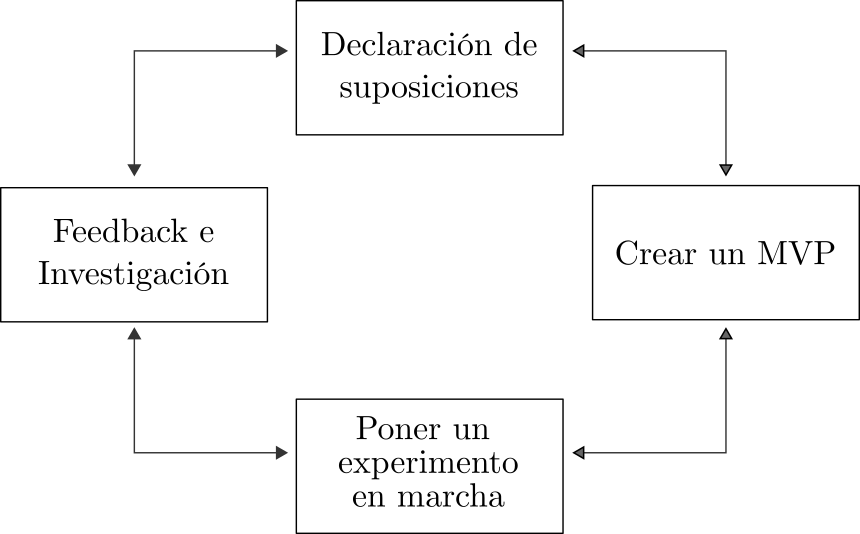
\includegraphics[width=10cm]{Img/Desarrollo/desarrollo0.png}
\centering
\caption{\textbf{ \footnotesize{Proceso del enfoque LEAN UX. }}}
\end{figure}
\label{fig:leanux}

Lean UX funciona como una práctica para entender rápidamente la función de un producto. Para ello elije un camino colaborativo y multidisciplinario; reduce el énfasis por la documentación exhaustiva y aumenta el enfoque en la construcción de un entendimiento compartido del producto que está siendo diseñado. Como consecuencia de usar este enfoque se obtiene: un equipo que trabaja de forma colaborativa, iterativamente, reduciendo al mínimo los documentos entregables, enfocándose en el software funcional y en la retroalimentación con el usuario final.

\subsection{Principios de LEAN UX}
\textit{Lean UX} contiene en su núcleo un juego de principios clave, que abarcan el proceso de diseño, la colaboración, la gestión, etc., para que los equipos puedan sacarle el máximo provecho al enfoque propio de la metodología. Se consigue con ellos que los equipos se encaminen en la dirección correcta y sean especialmente útiles para implementar los procesos de Lean UX. Los procesos, sin duda se deben ajustar a cada proyecto, por ende los principios de utilizan como guía y no de forma obligatoria. Algunos de ellos serán más difíciles de implementar y su impacto será mayor. Los equipos adoptarán sin problema otros, pero, independientemente de las dificultades, todos ellos ayudan a crear una organización más colaborativa, multifuncional y adaptada a la realidad actual de los proyectos.\vskip

A continuación se detallan los principios:
\begin{itemize}
    \item \textbf{Principio: Equipos multifuncionales}\vskip 
    ¿De qué se trata? Los equipos multifuncionales deben incluir todas las disciplinas que intervienen en la creación del producto. La ingeniería del software, la gestión del producto, el diseño de interacciones, el diseño gráfico, la estrategia de contenidos y el control de calidad (QA), todas deben contar con representantes en ellos. Lean UX necesita que todos los que se dedican a estos campos colaboren intensamente, por lo que la implicación del equipo debe ser continua, desde el primer día del proyecto hasta el final.\vskip
    ¿Por qué hacerlo? Estos equipos, diversos en su constitución, evitan el desarrollo en cascada, con su proceso rígido de entregas de documentación. En su lugar, todos los campos aportan conocimiento mucho antes al proceso. Como la metodología promueve, además, que los miembros de los diferentes ámbitos hablen entre ellos, la eficacia del equipo aumenta.
    
\item \textbf{Principio: Pequeños, dedicados, coubicados }\vskip 
    ¿De qué se trata? Es necesario limitar el tamaño de los equipos, no deben ser mayores de diez personas, dedicados exclusivamente al proyecto y trabajando en el mismo lugar. \vskip
    ¿Por qué hacerlo? El beneficio de los equipos pequeños se resume en tres palabras: comunicación, concentración y camaradería. Así se comunica de forma sencilla sobre el estado del proyecto, de los cambios y del nuevo conocimiento que surja. La dedicación en exclusiva, por otra parte, hace que todos los miembros estén centrados en las mismas prioridades. Y además, trabajar en el mismo lugar hace las relaciones entre colegas sean más estrechas.
    
    \item \textbf{Principio: Equipos centrados en los problemas}\vskip
    ¿De qué se trata? Un equipo centrado en los problemas es un grupo que sabe que debe resolver el problema asignado y no limitarse a implementar un grupo de funciones. Este principio es una extensión lógica del anterior, que afirmaba que el progreso del proyecto dependía de los resultados.\vskip
    ¿Por qué hacerlo? Si se asignan problemas completos a un equipo se demuestra más confianza en las personas que lo conforman. Además, así se les permite llegar a sus propias soluciones, con lo que se consigue aumentar la sensación de pertenencia en el proyecto.
    
    \item \textbf{Principio: Eliminación del despilfarro}\vskip
    ¿De qué se trata? Una de los prácticas principales de \textit{Lean manufacturing} es la eliminación de todo lo que no contribuya a conseguir el objetivo final. En Lean UX, este objetivo final es la producción de mejores resultados, por lo que todo lo que no ayude a conseguirlos se considera despilfarro y debe eliminarse del proceso de trabajo del equipo.\vskip
    ¿Por qué hacerlo? Los recursos del equipo son limitados, por lo que cuanto más despilfarro se elimine, más rápido podrán producir sus miembros. En realidad, lo que los equipos necesitan es ser efectivos y trabajar en los retos adecuados. Si se elimina el despilfarro, la atención de los equipos estará centrada donde se debe.
    
    \item \textbf{Principio: Lotes pequeños}\vskip
    ¿De qué se trata? Otra idea fundamental de \textit{Lean manufacturing} es la utilización de lotes pequeños. En ese modelo, esta noción se usa para indicar que no se deben tener muchos productos en stock y que la calidad de producción debía ser alta. Adaptado a Lean UX, su significado es que el equipo solo debe crear los diseños necesarios para avanzar, evitando crear un gran stock de ideas de diseño sin probar ni implementar. \vskip
    ¿Por qué hacerlo? El diseño en grandes lotes resta eficiencia al equipo, ya que, para poder realizar grandes entregas de diseño, se insume mucho tiempo. En ese tiempo no se puede aprender si las ideas funcionan e, inevitablemente, algunos de los miembros tendrán que estar desocupados, aparte de generar recursos de diseño inútiles. Es decir, se trata de una estrategia con un despilfarro que no maximiza el potencial de aprendizaje del equipo.
    
    \item \textbf{Principio: Descubrimiento continuo }\vskip
    ¿De qué se trata? El descubrimiento continuo consiste en comprometer a los usuarios con el proceso de diseño y desarrollo, mediante actividades programadas con ellos en intervalos regulares, en las que se aplican métodos cualitativos y cuantitativos. El objetivo es entender lo que los usuarios hacen con productos y por qué lo hacen. La investigación con ellos debe realizarse de forma frecuente y regular y debe implicar al todo el equipo.\vskip
    ¿Por qué hacerlo? Las conversaciones regulares con los usuarios ofrecen oportunidades de validar nuevas ideas sobre el producto. Por otra parte, al incluir al equipo completo en el ciclo de desarrollo, estos desarrollarán empatía por los usuarios y por los problemas a los que tienen que enfrentarse. Además, como todos los miembros aprenden juntos en las reuniones, no será necesario generar demasiada documentación ni explicar lo sucedido en otras reuniones internas.
    
    \item \textbf{Principio: GOOB: La nueva centralidad del usuario}\vskip
    ¿De qué se trata? Se utiliza el acrónimo \textit{Salir del edificio} en ingles \textit{Getting Out Of the Building} (GOOB). Quiere decir que los debates sobre las necesidades de los usuarios no tienen por qué cerrarse en el mismo lugar en el que se desarrollan, es decir, en la oficina. Las respuestas, más bien, están en el mercado, fuera de ella. Después de mucho tiempo abogando por la investigación del comportamiento de los usuarios, la comunidad de experiencia de usuarios (UX) tiene un aliado en Steve Blank, que viene del mundo de los negocios. Su consejo: Ofrecer la posibilidad a los usuarios de dar su opinión sobre las ideas mucho antes de lo que lo han hecho en el pasado. Mucho antes. Brindar nociones de la realidad mientras aún se está en etapas prematuras de desarrollo. Es mucho mejor averiguar que las ideas no son correctas mucho antes de dedicar tiempo y recursos a construir un producto que nadie quiere o necesota.\vskip
    ¿Por qué hacerlo? En los últimos tiempos, el éxito o el fracaso de los productos no dependen de las decisiones del equipo de desarrollo, sino de los usuarios. Son ellos los que tendrán que utilizar los producto. Cuanto antes se los haga participar, antes se aprende si las ideas están listas para pasar a la fase de desarrollo.

    \item \textbf{Principio: Entendimiento común}\vskip 
    ¿De qué se trata? El entendimiento común es el conocimiento colectivo del equipo. Se construye poco a poco a medida que ese equipo trabaja de forma conjunta y consiste en una comprensión profunda del espacio, del producto y de los clientes.\vskip 
    ¿Por qué hacerlo? Este tipo de conocimiento es la moneda de cambio de Lean UX. Cuanto más sepa el equipo, como colectivo, de lo que está haciendo y de por qué lo está haciendo, menos dependerá de informes de segunda mano y de documentos detallados para continuar con su trabajo.
    
    \item \textbf{Principio: Antimodelos: estrellas, gurús y ninjas }\vskip 
    ¿De qué se trata? Lean UX aboga por una mentalidad de equipo. Las estrellas, los gurús, los ninjas y, en general, rompen la cohesión del equipo y reducen la colaboración.\vskip ¿Por qué hacerlo? Las estrellas no comparten las ideas ni la atención de los demás. Si se cuenta con individuos de este tipo en los equipos, con grandes egos y determinados a brillar por encima de todos, se rompe la colaboración del grupo. Si eso sucede no se cuenta con un entorno en el que se pueda construir un entendimiento común, necesario para avanzar de forma efectiva.
    
    \item \textbf{Principio:Exteriorización del trabajo}\vskip
    ¿De qué se trata? Con exteriorización me refiero a exponer el trabajo de forma pública, más allá de las computadoras. Los equipos pueden utilizar pizarras, tableros de cartón, paredes repletas de artefactos, salidas impresas, notas adhesivas, lo que sea que hayan utilizado para reflejar sus ideas, para poder mostrar el trabajo a compañeros, colegas y clientes.\vskip 
    ¿Por qué hacerlo? La exteriorización somete las ideas a escrutinio público y así todos los miembros del equipo pueden ver dónde se encuentran como grupo. De esta manera se crea un flujo de información que circula entre todos los miembros, información que está en el ambiente y que inspira nuevas ideas, construidas sobre las que se han compartido. Además, esta forma de trabajar hace participar a todos los miembros del equipo, incluso las personas tímidas, ya que las notas adhesivas, se tratan por igual.

    \item \textbf{Principio: Aprendizaje en lugar de crecimiento}\vskip
    ¿De qué se trata? Es complicado concebir una buena idea y hacerla crecer al mismo tiempo. Son actividades contradictorias. Lean UX apuesta por que, en primer lugar, se concentre en el aprendizaje y luego en su crecimiento.\vskip 
    ¿Por qué hacerlo? Escalar una idea que no se ha probado es arriesgado. Podría funcionar o podría no hacerlo. Si no lo hace y la idea se sube a producción para todos los usuario, en lugar de para unos cuantos con los que probar, el equipo habrá perdido tiempo y recursos valiosos en hacerlo. Al asegurarse de que una idea funciona antes de hacerla crecer, se reduce el riesgo que conllevan los grandes despliegues de funciones.
    
    \item \textbf{Principio: Permiso para equivocarse}\vskip
    ¿De qué se trata? Para encontrar las mejores soluciones a los problemas, los equipos Lean UX necesitan experimentar con las ideas. La mayoría de estas ideas no funcionarán en primera instancia, por lo que, si se necesita que sean exitosas, el equipo debe sentirse libre para equivocarse. Este permiso significa que puede contar con un entorno seguro en el que experimentar, una filosofía que se debe aplicar tanto al entorno técnico (deben ser capaces de generar ideas en un entorno seguro) como al cultural (nadie debe penalizar a un miembro del equipo por probar ideas que no funcionen).\vskip 
    ¿Por qué hacerlo? El permiso para equivocarse alimenta la cultura de la experimentación que, a su vez, da alas a la creatividad. La creatividad, por su parte, hace que aparezcan soluciones innovadoras. Cuando, al equivocarse, los equipos no tienen miedo de ser penalizados, estarán dispuestos a correr riesgos. Y las grandes ideas siempre proceden de los riesgos.
    
    \item \textbf{Principio: Escapar de los negocios basados en entregables }\vskip
    ¿De qué se trata? El progreso de un proyecto depende de los resultados que se consiguen, no de los documentos que el equipo escriba. Por otra parte, la colaboración multifuncional permite conseguir que los participantes del proyecto tengan más en cuenta los resultados y menos los artefactos que se estén creando.\vskip 
    ¿Por qué hacerlo? Los documentos no solucionan los problemas de los usuarios; lo hacen los buenos productos. La atención del equipo debe estar enfocada en qué funciones de las que está desarrollando tienen mayor impacto. Los procedimientos que el equipo utilice para llegar a ese conocimiento son irrelevantes. Lo que importa es la calidad del producto, medida como la reacción que el usuario presenta ante él.
    
\end{itemize}



Los principios fundacionales de Lean UX tratan de los atributos principales que debe tener cualquier equipo que trabaje con esta metodología.
Por todo lo señalado se considera que este enfoque es el adecuado para abordar el trabajo en la aplicación COCADA para los métodos de trabajo en equipo.
Las etapas de LEAN UX se pueden ver aplicadas en este documento en el siguiente capítulo correspondiente al desarrollo del prototipo.



Agregar lo de chaos report http://www.laboratorioti.com/2016/05/16/informe-del-caos-2015-chaos-report-2015-bien-mal-fueron-los-proyectos-ano-2015/

https://modelometodoygestion.wordpress.com/2017/02/21/chaos-report-15-scrum/

Ver frase final para chamu
http://www.uxline.com/blog/agile-ux-versus-lean-ux/



VER LO DE FUZZY DESIGN y agregar tambien a la parte de codiseño

https://blog.prototypr.io/the-teapot-model-how-to-explain-a-fuzzy-design-process-to-anxious-clients-4a2e8487bc87


COMO ENGANCHAR TODO
https://es.linkedin.com/pulse/design-thinking-lean-startup-agile-victor-mansilla


https://www.cio.com/article/3174516/project-management/it-project-success-rates-finally-improving.html



https://www.pmi.org/-/media/pmi/documents/public/pdf/learning/thought-leadership/pulse/pulse-of-the-profession-2017.pdf